\documentclass{article} 
\usepackage[utf8]{inputenc}
 \usepackage{tikz}
 \usetikzlibrary{calc}
\begin{document} 
\pagestyle{empty}
    
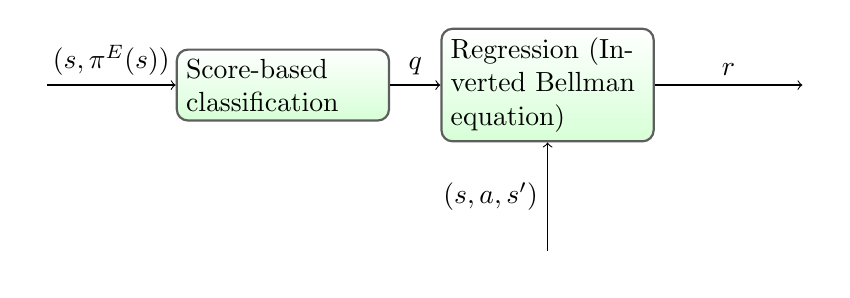
\begin{tikzpicture} [
  etape/.style=
  {rectangle,rounded corners, shade, top color=white,
    bottom color=green!80!white!20,
    draw=white!30!black!90,thick}]
\node (pseudoLeft) at (0,0){};
\node [etape,text width=7em] (classif) at ($(pseudoLeft.east)+(3,0)$) {Score-based classification };
\node [etape,text width=7em] (regression) at ($(classif.east)+(2,0)$) {Regression (Inverted Bellman equation)};
\node (pseudoBottom) at ($(regression.south)+(0,-1.5)$) {};
\node  (pseudoRight) at ($(regression.east)+(2,0)$) {};
\draw [->] (pseudoLeft) -- node[above]{$(s,\pi^E(s))$}  (classif.west);
\draw [->] (classif.east) -- node[above]{$q$}  (regression.west);
\draw [->] (regression.east) -- node[above]{$r$}  (pseudoRight);
\draw [->] (pseudoBottom) -- node[left]{$(s,a,s')$}  (regression.south);

\end{tikzpicture} 

\end{document}
% (launch-RTE)
